\documentclass[tikz,border=5pt]{standalone}
\usepackage[T1]{fontenc}
\usepackage{amsmath,amssymb}
\usepackage{newtxtext,newtxmath}
\usetikzlibrary{arrows.meta,calc}

\definecolor{Ink}{HTML}{202428}
\definecolor{SoftInk}{HTML}{666D73}
\definecolor{Probe}{HTML}{D99A00}
\definecolor{ProbePale}{HTML}{F7E8BB}
\definecolor{Common}{HTML}{2878B5}
\definecolor{Faraday}{HTML}{168866}
\definecolor{Cloud}{HTML}{D7DBDE}
\definecolor{OutputPale}{HTML}{E7E9EA}
\definecolor{Panel}{HTML}{FAFAFA}

\tikzset{
  >=Latex,
  every node/.style={text=Ink},
  panel/.style={rounded corners=2mm, draw=black!13, fill=Panel, line width=0.55pt},
}

\begin{document}
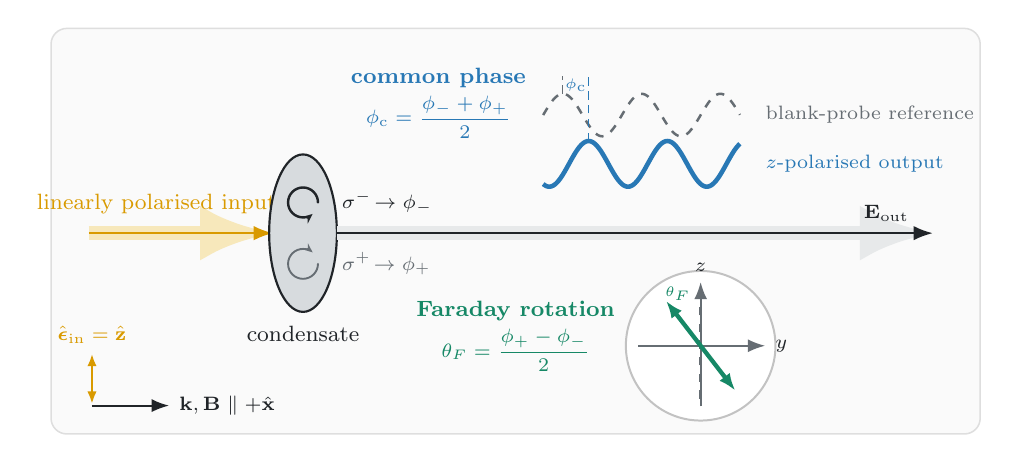
\begin{tikzpicture}[x=1cm,y=1cm]
  \path[panel] (0,0) rectangle (11.80,5.15);

  % One linearly polarised probe enters the condensate.
  \draw[-Latex, draw=ProbePale, line width=5.2pt] (0.48,2.55) -- (2.82,2.55);
  \draw[-Latex, draw=Probe, line width=0.9pt] (0.48,2.55) -- (2.82,2.55);
  \node[font=\footnotesize, text=Probe] at (1.34,2.92)
    {linearly polarised input};

  % Condensate and its two circular-polarisation eigenresponses.
  \coordinate (cloud) at (3.20,2.55);
  \draw[fill=Cloud, draw=Ink, line width=0.78pt]
    (cloud) ellipse [x radius=0.43, y radius=1.00];
  \node[font=\footnotesize] at (3.20,1.27) {condensate};

  \begin{scope}[shift={(3.20,2.94)}]
    \draw[-{Stealth[length=1.25mm,width=1.05mm]}, draw=Ink,
      line width=0.88pt, line cap=round]
      (0.19,0) arc[start angle=0,end angle=310,radius=0.19];
    \node[font=\scriptsize, anchor=west] at (0.37,0)
      {$\sigma^-\!\rightarrow\phi_-$};
  \end{scope}
  \begin{scope}[shift={(3.20,2.16)}]
    \draw[-{Stealth[length=1.18mm,width=0.98mm]}, draw=SoftInk,
      line width=0.68pt, line cap=round]
      (0.19,0) arc[start angle=0,end angle=-310,radius=0.19];
    \node[font=\scriptsize, anchor=west, text=SoftInk] at (0.37,0)
      {$\sigma^+\!\rightarrow\phi_+$};
  \end{scope}

  % The output remains one transmitted probe; it is not split into coloured beams.
  \draw[-Latex, draw=OutputPale, line width=5.2pt] (3.63,2.55) -- (11.20,2.55);
  \draw[-Latex, draw=Ink, line width=0.88pt] (3.63,2.55) -- (11.20,2.55);
  \node[font=\scriptsize, anchor=east] at (11.02,2.80)
    {$\mathbf E_{\mathrm{out}}$};

  % Common phase: compare the z-polarised output with the no-atom phase reference.
  \node[font=\bfseries\footnotesize, text=Common] at (4.92,4.52)
    {common phase};
  \node[font=\scriptsize, text=Common] at (4.92,4.02)
    {$\displaystyle \phi_{\mathrm c}=\frac{\phi_-+\phi_+}{2}$};
  \draw[draw=SoftInk, dashed, line width=0.90pt]
    plot[domain=6.25:8.75,samples=140]
    (\x,{4.05+0.27*sin(360*(\x-6.25))});
  \draw[draw=Common, line width=1.65pt]
    plot[domain=6.25:8.75,samples=140]
    (\x,{3.43+0.29*sin(360*(\x-6.25)-118)});
  \draw[draw=SoftInk, densely dashed, line width=0.34pt]
    (6.50,4.32) -- (6.50,4.55);
  \draw[draw=Common, densely dashed, line width=0.34pt]
    (6.83,3.72) -- (6.83,4.55);
  \node[font=\tiny, text=Common] at (6.665,4.43) {$\phi_{\mathrm c}$};
  \node[font=\scriptsize, text=SoftInk, anchor=west] at (8.95,4.05)
    {blank-probe reference};
  \node[font=\scriptsize, text=Common, anchor=west] at (8.95,3.43)
    {$z$-polarised output};

  % Faraday rotation: the output polarisation turns relative to the input axis.
  \node[font=\bfseries\footnotesize, text=Faraday] at (5.90,1.56)
    {Faraday rotation};
  \node[font=\scriptsize, text=Faraday] at (5.90,1.06)
    {$\displaystyle \theta_F=\frac{\phi_+-\phi_-}{2}$};
  \begin{scope}[shift={(8.25,1.12)}]
    \draw[draw=black!24, fill=white, line width=0.72pt]
      (0,0) circle[radius=0.95];
    \draw[-Latex, draw=SoftInk, line width=0.72pt] (0,-0.77) -- (0,0.81)
      node[above, font=\scriptsize] {$z$};
    \draw[-Latex, draw=SoftInk, line width=0.72pt] (-0.79,0) -- (0.82,0)
      node[right, font=\scriptsize] {$y$};
    \draw[draw=SoftInk, dashed, line width=0.86pt] (0,-0.67) -- (0,0.67);
    \draw[{Latex[length=2.2mm]}-{Latex[length=2.2mm]}, draw=Faraday,
      line width=1.55pt] (0.44,-0.57) -- (-0.44,0.57);
    \node[font=\tiny, text=Faraday] at (-0.29,0.66) {$\theta_F$};
  \end{scope}

  % Compact geometry marker.
  \coordinate (geom) at (0.52,0.36);
  \draw[-Latex, draw=Ink, line width=0.75pt] (geom) -- ++(0.98,0)
    node[right, font=\scriptsize] {$\mathbf k,\mathbf B\parallel+\hat{\mathbf x}$};
  \draw[{Latex[length=1.6mm]}-{Latex[length=1.6mm]}, draw=Probe, line width=1.0pt]
    ($(geom)+(0,0.02)$) -- ++(0,0.64)
    node[above, font=\scriptsize, text=Probe]
    {$\hat{\boldsymbol\epsilon}_{\rm in}=\hat{\mathbf z}$};
\end{tikzpicture}
\end{document}
